% !TEX encoding = UTF-8 Unicode
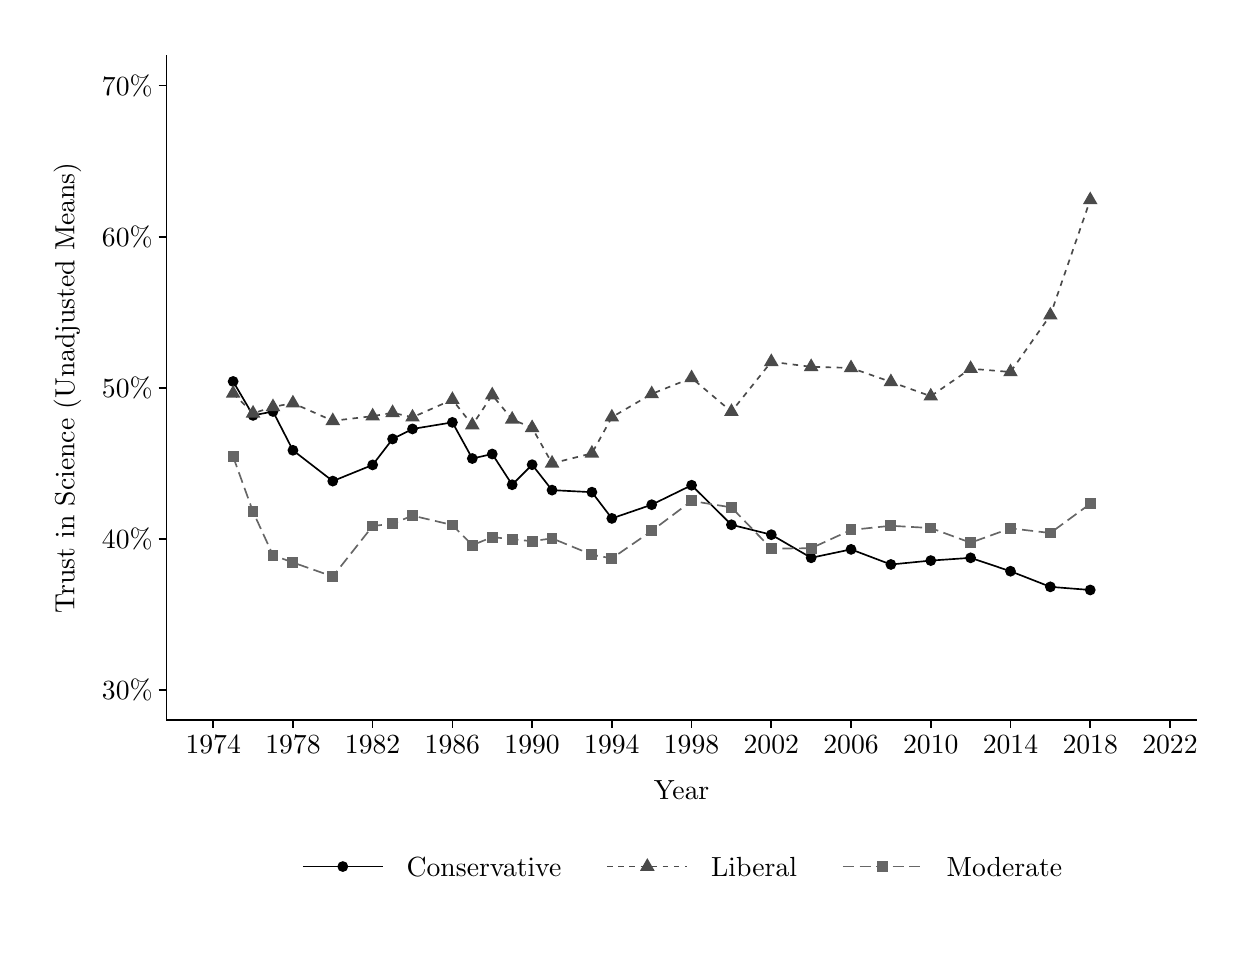
\begin{tikzpicture}[x=1pt,y=1pt]
\definecolor{fillColor}{RGB}{255,255,255}
\path[use as bounding box,fill=fillColor,fill opacity=0.00] (0,0) rectangle (432.48,324.36);
\begin{scope}
\path[clip] (  0.00,  0.00) rectangle (432.48,324.36);
\definecolor{fillColor}{RGB}{255,255,255}

\path[fill=fillColor] ( -0.00,  0.00) rectangle (432.48,324.36);
\end{scope}
\begin{scope}
\path[clip] ( 50.11, 74.07) rectangle (422.48,314.36);
\definecolor{fillColor}{RGB}{255,255,255}

\path[fill=fillColor] ( 50.11, 74.07) rectangle (422.48,314.36);
\definecolor{drawColor}{RGB}{0,0,0}

\path[draw=drawColor,line width= 0.6pt,line join=round] ( 74.24,196.52) --
	( 81.44,184.25) --
	( 88.64,185.66) --
	( 95.85,171.64) --
	(110.25,160.51) --
	(124.66,166.36) --
	(131.86,175.73) --
	(139.06,179.36) --
	(153.47,181.73) --
	(160.67,168.67) --
	(167.87,170.30) --
	(175.07,159.19) --
	(182.28,166.44) --
	(189.48,157.25) --
	(203.88,156.51) --
	(211.09,147.03) --
	(225.49,151.98) --
	(239.90,159.02) --
	(254.30,144.73) --
	(268.71,141.15) --
	(283.11,132.80) --
	(297.52,135.84) --
	(311.92,130.38) --
	(326.33,131.79) --
	(340.73,132.78) --
	(355.14,127.94) --
	(369.54,122.30) --
	(383.95,121.17);
\definecolor{drawColor}{gray}{0.29}

\path[draw=drawColor,line width= 0.6pt,dash pattern=on 2pt off 2pt ,line join=round] ( 74.24,192.20) --
	( 81.44,185.01) --
	( 88.64,187.33) --
	( 95.85,188.68) --
	(110.25,182.30) --
	(124.66,183.98) --
	(131.86,185.20) --
	(139.06,183.58) --
	(153.47,189.94) --
	(160.67,180.75) --
	(167.87,191.59) --
	(175.07,182.82) --
	(182.28,179.77) --
	(189.48,166.93) --
	(203.88,170.53) --
	(211.09,183.60) --
	(225.49,192.01) --
	(239.90,197.78) --
	(254.30,185.61) --
	(268.71,203.63) --
	(283.11,201.81) --
	(297.52,201.40) --
	(311.92,196.36) --
	(326.33,191.19) --
	(340.73,201.13) --
	(355.14,199.94) --
	(369.54,220.43) --
	(383.95,262.10);
\definecolor{drawColor}{gray}{0.40}

\path[draw=drawColor,line width= 0.6pt,dash pattern=on 4pt off 2pt ,line join=round] ( 74.24,169.35) --
	( 81.44,149.41) --
	( 88.64,133.73) --
	( 95.85,131.10) --
	(110.25,126.03) --
	(124.66,144.28) --
	(131.86,145.11) --
	(139.06,148.04) --
	(153.47,144.64) --
	(160.67,137.36) --
	(167.87,140.27) --
	(175.07,139.51) --
	(182.28,138.79) --
	(189.48,139.82) --
	(203.88,133.92) --
	(211.09,132.58) --
	(225.49,142.51) --
	(239.90,153.34) --
	(254.30,151.01) --
	(268.71,136.12) --
	(283.11,136.25) --
	(297.52,142.87) --
	(311.92,144.37) --
	(326.33,143.55) --
	(340.73,138.25) --
	(355.14,143.44) --
	(369.54,141.76) --
	(383.95,152.31);
\definecolor{fillColor}{RGB}{0,0,0}

\path[fill=fillColor] ( 74.24,196.52) circle (  1.96);
\definecolor{fillColor}{gray}{0.29}

\path[fill=fillColor] ( 74.24,195.25) --
	( 76.88,190.68) --
	( 71.60,190.68) --
	cycle;
\definecolor{fillColor}{gray}{0.40}

\path[fill=fillColor] ( 72.28,167.39) --
	( 76.20,167.39) --
	( 76.20,171.31) --
	( 72.28,171.31) --
	cycle;
\definecolor{fillColor}{RGB}{0,0,0}

\path[fill=fillColor] ( 81.44,184.25) circle (  1.96);
\definecolor{fillColor}{gray}{0.29}

\path[fill=fillColor] ( 81.44,188.06) --
	( 84.08,183.48) --
	( 78.80,183.48) --
	cycle;
\definecolor{fillColor}{gray}{0.40}

\path[fill=fillColor] ( 79.48,147.44) --
	( 83.40,147.44) --
	( 83.40,151.37) --
	( 79.48,151.37) --
	cycle;
\definecolor{fillColor}{RGB}{0,0,0}

\path[fill=fillColor] ( 88.64,185.66) circle (  1.96);
\definecolor{fillColor}{gray}{0.29}

\path[fill=fillColor] ( 88.64,190.38) --
	( 91.29,185.80) --
	( 86.00,185.80) --
	cycle;
\definecolor{fillColor}{gray}{0.40}

\path[fill=fillColor] ( 86.68,131.77) --
	( 90.61,131.77) --
	( 90.61,135.70) --
	( 86.68,135.70) --
	cycle;
\definecolor{fillColor}{RGB}{0,0,0}

\path[fill=fillColor] ( 95.85,171.64) circle (  1.96);
\definecolor{fillColor}{gray}{0.29}

\path[fill=fillColor] ( 95.85,191.73) --
	( 98.49,187.15) --
	( 93.20,187.15) --
	cycle;
\definecolor{fillColor}{gray}{0.40}

\path[fill=fillColor] ( 93.88,129.14) --
	( 97.81,129.14) --
	( 97.81,133.06) --
	( 93.88,133.06) --
	cycle;
\definecolor{fillColor}{RGB}{0,0,0}

\path[fill=fillColor] (110.25,160.51) circle (  1.96);
\definecolor{fillColor}{gray}{0.29}

\path[fill=fillColor] (110.25,185.35) --
	(112.89,180.77) --
	(107.61,180.77) --
	cycle;
\definecolor{fillColor}{gray}{0.40}

\path[fill=fillColor] (108.29,124.07) --
	(112.21,124.07) --
	(112.21,127.99) --
	(108.29,127.99) --
	cycle;
\definecolor{fillColor}{RGB}{0,0,0}

\path[fill=fillColor] (124.66,166.36) circle (  1.96);
\definecolor{fillColor}{gray}{0.29}

\path[fill=fillColor] (124.66,187.03) --
	(127.30,182.46) --
	(122.01,182.46) --
	cycle;
\definecolor{fillColor}{gray}{0.40}

\path[fill=fillColor] (122.69,142.32) --
	(126.62,142.32) --
	(126.62,146.24) --
	(122.69,146.24) --
	cycle;
\definecolor{fillColor}{RGB}{0,0,0}

\path[fill=fillColor] (131.86,175.73) circle (  1.96);
\definecolor{fillColor}{gray}{0.29}

\path[fill=fillColor] (131.86,188.25) --
	(134.50,183.67) --
	(129.22,183.67) --
	cycle;
\definecolor{fillColor}{gray}{0.40}

\path[fill=fillColor] (129.90,143.15) --
	(133.82,143.15) --
	(133.82,147.07) --
	(129.90,147.07) --
	cycle;
\definecolor{fillColor}{RGB}{0,0,0}

\path[fill=fillColor] (139.06,179.36) circle (  1.96);
\definecolor{fillColor}{gray}{0.29}

\path[fill=fillColor] (139.06,186.64) --
	(141.70,182.06) --
	(136.42,182.06) --
	cycle;
\definecolor{fillColor}{gray}{0.40}

\path[fill=fillColor] (137.10,146.08) --
	(141.02,146.08) --
	(141.02,150.00) --
	(137.10,150.00) --
	cycle;
\definecolor{fillColor}{RGB}{0,0,0}

\path[fill=fillColor] (153.47,181.73) circle (  1.96);
\definecolor{fillColor}{gray}{0.29}

\path[fill=fillColor] (153.47,192.99) --
	(156.11,188.41) --
	(150.82,188.41) --
	cycle;
\definecolor{fillColor}{gray}{0.40}

\path[fill=fillColor] (151.50,142.68) --
	(155.43,142.68) --
	(155.43,146.61) --
	(151.50,146.61) --
	cycle;
\definecolor{fillColor}{RGB}{0,0,0}

\path[fill=fillColor] (160.67,168.67) circle (  1.96);
\definecolor{fillColor}{gray}{0.29}

\path[fill=fillColor] (160.67,183.80) --
	(163.31,179.22) --
	(158.03,179.22) --
	cycle;
\definecolor{fillColor}{gray}{0.40}

\path[fill=fillColor] (158.71,135.40) --
	(162.63,135.40) --
	(162.63,139.32) --
	(158.71,139.32) --
	cycle;
\definecolor{fillColor}{RGB}{0,0,0}

\path[fill=fillColor] (167.87,170.30) circle (  1.96);
\definecolor{fillColor}{gray}{0.29}

\path[fill=fillColor] (167.87,194.64) --
	(170.51,190.06) --
	(165.23,190.06) --
	cycle;
\definecolor{fillColor}{gray}{0.40}

\path[fill=fillColor] (165.91,138.31) --
	(169.83,138.31) --
	(169.83,142.23) --
	(165.91,142.23) --
	cycle;
\definecolor{fillColor}{RGB}{0,0,0}

\path[fill=fillColor] (175.07,159.19) circle (  1.96);
\definecolor{fillColor}{gray}{0.29}

\path[fill=fillColor] (175.07,185.87) --
	(177.72,181.29) --
	(172.43,181.29) --
	cycle;
\definecolor{fillColor}{gray}{0.40}

\path[fill=fillColor] (173.11,137.54) --
	(177.04,137.54) --
	(177.04,141.47) --
	(173.11,141.47) --
	cycle;
\definecolor{fillColor}{RGB}{0,0,0}

\path[fill=fillColor] (182.28,166.44) circle (  1.96);
\definecolor{fillColor}{gray}{0.29}

\path[fill=fillColor] (182.28,182.82) --
	(184.92,178.24) --
	(179.63,178.24) --
	cycle;
\definecolor{fillColor}{gray}{0.40}

\path[fill=fillColor] (180.31,136.83) --
	(184.24,136.83) --
	(184.24,140.76) --
	(180.31,140.76) --
	cycle;
\definecolor{fillColor}{RGB}{0,0,0}

\path[fill=fillColor] (189.48,157.25) circle (  1.96);
\definecolor{fillColor}{gray}{0.29}

\path[fill=fillColor] (189.48,169.98) --
	(192.12,165.41) --
	(186.84,165.41) --
	cycle;
\definecolor{fillColor}{gray}{0.40}

\path[fill=fillColor] (187.52,137.86) --
	(191.44,137.86) --
	(191.44,141.79) --
	(187.52,141.79) --
	cycle;
\definecolor{fillColor}{RGB}{0,0,0}

\path[fill=fillColor] (203.88,156.51) circle (  1.96);
\definecolor{fillColor}{gray}{0.29}

\path[fill=fillColor] (203.88,173.58) --
	(206.53,169.01) --
	(201.24,169.01) --
	cycle;
\definecolor{fillColor}{gray}{0.40}

\path[fill=fillColor] (201.92,131.96) --
	(205.85,131.96) --
	(205.85,135.89) --
	(201.92,135.89) --
	cycle;
\definecolor{fillColor}{RGB}{0,0,0}

\path[fill=fillColor] (211.09,147.03) circle (  1.96);
\definecolor{fillColor}{gray}{0.29}

\path[fill=fillColor] (211.09,186.65) --
	(213.73,182.08) --
	(208.44,182.08) --
	cycle;
\definecolor{fillColor}{gray}{0.40}

\path[fill=fillColor] (209.12,130.62) --
	(213.05,130.62) --
	(213.05,134.54) --
	(209.12,134.54) --
	cycle;
\definecolor{fillColor}{RGB}{0,0,0}

\path[fill=fillColor] (225.49,151.98) circle (  1.96);
\definecolor{fillColor}{gray}{0.29}

\path[fill=fillColor] (225.49,195.06) --
	(228.13,190.48) --
	(222.85,190.48) --
	cycle;
\definecolor{fillColor}{gray}{0.40}

\path[fill=fillColor] (223.53,140.54) --
	(227.45,140.54) --
	(227.45,144.47) --
	(223.53,144.47) --
	cycle;
\definecolor{fillColor}{RGB}{0,0,0}

\path[fill=fillColor] (239.90,159.02) circle (  1.96);
\definecolor{fillColor}{gray}{0.29}

\path[fill=fillColor] (239.90,200.83) --
	(242.54,196.25) --
	(237.25,196.25) --
	cycle;
\definecolor{fillColor}{gray}{0.40}

\path[fill=fillColor] (237.94,151.38) --
	(241.86,151.38) --
	(241.86,155.31) --
	(237.94,155.31) --
	cycle;
\definecolor{fillColor}{RGB}{0,0,0}

\path[fill=fillColor] (254.30,144.73) circle (  1.96);
\definecolor{fillColor}{gray}{0.29}

\path[fill=fillColor] (254.30,188.66) --
	(256.94,184.09) --
	(251.66,184.09) --
	cycle;
\definecolor{fillColor}{gray}{0.40}

\path[fill=fillColor] (252.34,149.04) --
	(256.26,149.04) --
	(256.26,152.97) --
	(252.34,152.97) --
	cycle;
\definecolor{fillColor}{RGB}{0,0,0}

\path[fill=fillColor] (268.71,141.15) circle (  1.96);
\definecolor{fillColor}{gray}{0.29}

\path[fill=fillColor] (268.71,206.68) --
	(271.35,202.10) --
	(266.06,202.10) --
	cycle;
\definecolor{fillColor}{gray}{0.40}

\path[fill=fillColor] (266.75,134.16) --
	(270.67,134.16) --
	(270.67,138.08) --
	(266.75,138.08) --
	cycle;
\definecolor{fillColor}{RGB}{0,0,0}

\path[fill=fillColor] (283.11,132.80) circle (  1.96);
\definecolor{fillColor}{gray}{0.29}

\path[fill=fillColor] (283.11,204.87) --
	(285.76,200.29) --
	(280.47,200.29) --
	cycle;
\definecolor{fillColor}{gray}{0.40}

\path[fill=fillColor] (281.15,134.28) --
	(285.07,134.28) --
	(285.07,138.21) --
	(281.15,138.21) --
	cycle;
\definecolor{fillColor}{RGB}{0,0,0}

\path[fill=fillColor] (297.52,135.84) circle (  1.96);
\definecolor{fillColor}{gray}{0.29}

\path[fill=fillColor] (297.52,204.45) --
	(300.16,199.87) --
	(294.88,199.87) --
	cycle;
\definecolor{fillColor}{gray}{0.40}

\path[fill=fillColor] (295.56,140.90) --
	(299.48,140.90) --
	(299.48,144.83) --
	(295.56,144.83) --
	cycle;
\definecolor{fillColor}{RGB}{0,0,0}

\path[fill=fillColor] (311.92,130.38) circle (  1.96);
\definecolor{fillColor}{gray}{0.29}

\path[fill=fillColor] (311.92,199.41) --
	(314.57,194.83) --
	(309.28,194.83) --
	cycle;
\definecolor{fillColor}{gray}{0.40}

\path[fill=fillColor] (309.96,142.41) --
	(313.88,142.41) --
	(313.88,146.33) --
	(309.96,146.33) --
	cycle;
\definecolor{fillColor}{RGB}{0,0,0}

\path[fill=fillColor] (326.33,131.79) circle (  1.96);
\definecolor{fillColor}{gray}{0.29}

\path[fill=fillColor] (326.33,194.24) --
	(328.97,189.66) --
	(323.69,189.66) --
	cycle;
\definecolor{fillColor}{gray}{0.40}

\path[fill=fillColor] (324.37,141.59) --
	(328.29,141.59) --
	(328.29,145.51) --
	(324.37,145.51) --
	cycle;
\definecolor{fillColor}{RGB}{0,0,0}

\path[fill=fillColor] (340.73,132.78) circle (  1.96);
\definecolor{fillColor}{gray}{0.29}

\path[fill=fillColor] (340.73,204.18) --
	(343.38,199.60) --
	(338.09,199.60) --
	cycle;
\definecolor{fillColor}{gray}{0.40}

\path[fill=fillColor] (338.77,136.29) --
	(342.70,136.29) --
	(342.70,140.21) --
	(338.77,140.21) --
	cycle;
\definecolor{fillColor}{RGB}{0,0,0}

\path[fill=fillColor] (355.14,127.94) circle (  1.96);
\definecolor{fillColor}{gray}{0.29}

\path[fill=fillColor] (355.14,202.99) --
	(357.78,198.41) --
	(352.50,198.41) --
	cycle;
\definecolor{fillColor}{gray}{0.40}

\path[fill=fillColor] (353.18,141.48) --
	(357.10,141.48) --
	(357.10,145.40) --
	(353.18,145.40) --
	cycle;
\definecolor{fillColor}{RGB}{0,0,0}

\path[fill=fillColor] (369.54,122.30) circle (  1.96);
\definecolor{fillColor}{gray}{0.29}

\path[fill=fillColor] (369.54,223.48) --
	(372.19,218.91) --
	(366.90,218.91) --
	cycle;
\definecolor{fillColor}{gray}{0.40}

\path[fill=fillColor] (367.58,139.80) --
	(371.51,139.80) --
	(371.51,143.72) --
	(367.58,143.72) --
	cycle;
\definecolor{fillColor}{RGB}{0,0,0}

\path[fill=fillColor] (383.95,121.17) circle (  1.96);
\definecolor{fillColor}{gray}{0.29}

\path[fill=fillColor] (383.95,265.16) --
	(386.59,260.58) --
	(381.31,260.58) --
	cycle;
\definecolor{fillColor}{gray}{0.40}

\path[fill=fillColor] (381.99,150.34) --
	(385.91,150.34) --
	(385.91,154.27) --
	(381.99,154.27) --
	cycle;
\end{scope}
\begin{scope}
\path[clip] (  0.00,  0.00) rectangle (432.48,324.36);
\definecolor{drawColor}{RGB}{0,0,0}

\path[draw=drawColor,line width= 0.6pt,line join=round] ( 50.11, 74.07) --
	( 50.11,314.36);
\end{scope}
\begin{scope}
\path[clip] (  0.00,  0.00) rectangle (432.48,324.36);
\definecolor{drawColor}{RGB}{0,0,0}

\node[text=drawColor,anchor=base east,inner sep=0pt, outer sep=0pt, scale=  1.00] at ( 45.16, 81.55) {30{\%}};

\node[text=drawColor,anchor=base east,inner sep=0pt, outer sep=0pt, scale=  1.00] at ( 45.16,136.16) {40{\%}};

\node[text=drawColor,anchor=base east,inner sep=0pt, outer sep=0pt, scale=  1.00] at ( 45.16,190.77) {50{\%}};

\node[text=drawColor,anchor=base east,inner sep=0pt, outer sep=0pt, scale=  1.00] at ( 45.16,245.38) {60{\%}};

\node[text=drawColor,anchor=base east,inner sep=0pt, outer sep=0pt, scale=  1.00] at ( 45.16,300.00) {70{\%}};
\end{scope}
\begin{scope}
\path[clip] (  0.00,  0.00) rectangle (432.48,324.36);
\definecolor{drawColor}{RGB}{0,0,0}

\path[draw=drawColor,line width= 0.6pt,line join=round] ( 47.36, 84.99) --
	( 50.11, 84.99);

\path[draw=drawColor,line width= 0.6pt,line join=round] ( 47.36,139.60) --
	( 50.11,139.60);

\path[draw=drawColor,line width= 0.6pt,line join=round] ( 47.36,194.21) --
	( 50.11,194.21);

\path[draw=drawColor,line width= 0.6pt,line join=round] ( 47.36,248.83) --
	( 50.11,248.83);

\path[draw=drawColor,line width= 0.6pt,line join=round] ( 47.36,303.44) --
	( 50.11,303.44);
\end{scope}
\begin{scope}
\path[clip] (  0.00,  0.00) rectangle (432.48,324.36);
\definecolor{drawColor}{RGB}{0,0,0}

\path[draw=drawColor,line width= 0.6pt,line join=round] ( 50.11, 74.07) --
	(422.48, 74.07);
\end{scope}
\begin{scope}
\path[clip] (  0.00,  0.00) rectangle (432.48,324.36);
\definecolor{drawColor}{RGB}{0,0,0}

\path[draw=drawColor,line width= 0.6pt,line join=round] ( 67.04, 71.32) --
	( 67.04, 74.07);

\path[draw=drawColor,line width= 0.6pt,line join=round] ( 95.85, 71.32) --
	( 95.85, 74.07);

\path[draw=drawColor,line width= 0.6pt,line join=round] (124.66, 71.32) --
	(124.66, 74.07);

\path[draw=drawColor,line width= 0.6pt,line join=round] (153.47, 71.32) --
	(153.47, 74.07);

\path[draw=drawColor,line width= 0.6pt,line join=round] (182.28, 71.32) --
	(182.28, 74.07);

\path[draw=drawColor,line width= 0.6pt,line join=round] (211.09, 71.32) --
	(211.09, 74.07);

\path[draw=drawColor,line width= 0.6pt,line join=round] (239.90, 71.32) --
	(239.90, 74.07);

\path[draw=drawColor,line width= 0.6pt,line join=round] (268.71, 71.32) --
	(268.71, 74.07);

\path[draw=drawColor,line width= 0.6pt,line join=round] (297.52, 71.32) --
	(297.52, 74.07);

\path[draw=drawColor,line width= 0.6pt,line join=round] (326.33, 71.32) --
	(326.33, 74.07);

\path[draw=drawColor,line width= 0.6pt,line join=round] (355.14, 71.32) --
	(355.14, 74.07);

\path[draw=drawColor,line width= 0.6pt,line join=round] (383.95, 71.32) --
	(383.95, 74.07);

\path[draw=drawColor,line width= 0.6pt,line join=round] (412.76, 71.32) --
	(412.76, 74.07);
\end{scope}
\begin{scope}
\path[clip] (  0.00,  0.00) rectangle (432.48,324.36);
\definecolor{drawColor}{RGB}{0,0,0}

\node[text=drawColor,anchor=base,inner sep=0pt, outer sep=0pt, scale=  1.00] at ( 67.04, 62.23) {1974};

\node[text=drawColor,anchor=base,inner sep=0pt, outer sep=0pt, scale=  1.00] at ( 95.85, 62.23) {1978};

\node[text=drawColor,anchor=base,inner sep=0pt, outer sep=0pt, scale=  1.00] at (124.66, 62.23) {1982};

\node[text=drawColor,anchor=base,inner sep=0pt, outer sep=0pt, scale=  1.00] at (153.47, 62.23) {1986};

\node[text=drawColor,anchor=base,inner sep=0pt, outer sep=0pt, scale=  1.00] at (182.28, 62.23) {1990};

\node[text=drawColor,anchor=base,inner sep=0pt, outer sep=0pt, scale=  1.00] at (211.09, 62.23) {1994};

\node[text=drawColor,anchor=base,inner sep=0pt, outer sep=0pt, scale=  1.00] at (239.90, 62.23) {1998};

\node[text=drawColor,anchor=base,inner sep=0pt, outer sep=0pt, scale=  1.00] at (268.71, 62.23) {2002};

\node[text=drawColor,anchor=base,inner sep=0pt, outer sep=0pt, scale=  1.00] at (297.52, 62.23) {2006};

\node[text=drawColor,anchor=base,inner sep=0pt, outer sep=0pt, scale=  1.00] at (326.33, 62.23) {2010};

\node[text=drawColor,anchor=base,inner sep=0pt, outer sep=0pt, scale=  1.00] at (355.14, 62.23) {2014};

\node[text=drawColor,anchor=base,inner sep=0pt, outer sep=0pt, scale=  1.00] at (383.95, 62.23) {2018};

\node[text=drawColor,anchor=base,inner sep=0pt, outer sep=0pt, scale=  1.00] at (412.76, 62.23) {2022};
\end{scope}
\begin{scope}
\path[clip] (  0.00,  0.00) rectangle (432.48,324.36);
\definecolor{drawColor}{RGB}{0,0,0}

\node[text=drawColor,anchor=base,inner sep=0pt, outer sep=0pt, scale=  1.00] at (236.30, 45.40) {Year};
\end{scope}
\begin{scope}
\path[clip] (  0.00,  0.00) rectangle (432.48,324.36);
\definecolor{drawColor}{RGB}{0,0,0}

\node[text=drawColor,rotate= 90.00,anchor=base,inner sep=0pt, outer sep=0pt, scale=  1.00] at ( 16.89,194.21) {Trust in Science (Unadjusted Means)};
\end{scope}
\begin{scope}
\path[clip] (  0.00,  0.00) rectangle (432.48,324.36);

\path[] ( 86.80, 10.00) rectangle (385.79, 32.45);
\end{scope}
\begin{scope}
\path[clip] (  0.00,  0.00) rectangle (432.48,324.36);

\path[] ( 95.80, 14.00) rectangle (131.94, 28.45);
\end{scope}
\begin{scope}
\path[clip] (  0.00,  0.00) rectangle (432.48,324.36);
\definecolor{drawColor}{RGB}{0,0,0}

\path[draw=drawColor,line width= 0.6pt,line join=round] ( 99.42, 21.23) -- (128.33, 21.23);
\end{scope}
\begin{scope}
\path[clip] (  0.00,  0.00) rectangle (432.48,324.36);
\definecolor{fillColor}{RGB}{0,0,0}

\path[fill=fillColor] (113.87, 21.23) circle (  1.96);
\end{scope}
\begin{scope}
\path[clip] (  0.00,  0.00) rectangle (432.48,324.36);

\path[] (205.84, 14.00) rectangle (241.98, 28.45);
\end{scope}
\begin{scope}
\path[clip] (  0.00,  0.00) rectangle (432.48,324.36);
\definecolor{drawColor}{gray}{0.29}

\path[draw=drawColor,line width= 0.6pt,dash pattern=on 2pt off 2pt ,line join=round] (209.46, 21.23) -- (238.36, 21.23);
\end{scope}
\begin{scope}
\path[clip] (  0.00,  0.00) rectangle (432.48,324.36);
\definecolor{fillColor}{gray}{0.29}

\path[fill=fillColor] (223.91, 24.28) --
	(226.55, 19.70) --
	(221.27, 19.70) --
	cycle;
\end{scope}
\begin{scope}
\path[clip] (  0.00,  0.00) rectangle (432.48,324.36);

\path[] (290.97, 14.00) rectangle (327.10, 28.45);
\end{scope}
\begin{scope}
\path[clip] (  0.00,  0.00) rectangle (432.48,324.36);
\definecolor{drawColor}{gray}{0.40}

\path[draw=drawColor,line width= 0.6pt,dash pattern=on 4pt off 2pt ,line join=round] (294.58, 21.23) -- (323.49, 21.23);
\end{scope}
\begin{scope}
\path[clip] (  0.00,  0.00) rectangle (432.48,324.36);
\definecolor{fillColor}{gray}{0.40}

\path[fill=fillColor] (307.07, 19.26) --
	(311.00, 19.26) --
	(311.00, 23.19) --
	(307.07, 23.19) --
	cycle;
\end{scope}
\begin{scope}
\path[clip] (  0.00,  0.00) rectangle (432.48,324.36);
\definecolor{drawColor}{RGB}{0,0,0}

\node[text=drawColor,anchor=base west,inner sep=0pt, outer sep=0pt, scale=  1.00] at (136.94, 17.78) {Conservative};
\end{scope}
\begin{scope}
\path[clip] (  0.00,  0.00) rectangle (432.48,324.36);
\definecolor{drawColor}{RGB}{0,0,0}

\node[text=drawColor,anchor=base west,inner sep=0pt, outer sep=0pt, scale=  1.00] at (246.98, 17.78) {Liberal};
\end{scope}
\begin{scope}
\path[clip] (  0.00,  0.00) rectangle (432.48,324.36);
\definecolor{drawColor}{RGB}{0,0,0}

\node[text=drawColor,anchor=base west,inner sep=0pt, outer sep=0pt, scale=  1.00] at (332.10, 17.78) {Moderate};
\end{scope}
\end{tikzpicture}
